%%%%%%%%%%%%%%%%%%%%%%%%%%%%%%%%%%%%%%%%%%%%%%%%%%%%%%%%%%%%%%%%%%%%
%% I, the copyright holder of this work, release this work into the
%% public domain. This applies worldwide. In some countries this may
%% not be legally possible; if so: I grant anyone the right to use
%% this work for any purpose, without any conditions, unless such
%% conditions are required by law.
%%%%%%%%%%%%%%%%%%%%%%%%%%%%%%%%%%%%%%%%%%%%%%%%%%%%%%%%%%%%%%%%%%%%

\documentclass[
  digital,     %% The `digital` option enables the default options for the
               %% digital version of a document. Replace with `printed`
               %% to enable the default options for the printed version
               %% of a document.
%%  color,       %% Uncomment these lines (by removing the %% at the
%%               %% beginning) to use color in the printed version of your
%%               %% document
  twoside,     %% The `twoside` option enables double-sided typesetting.
               %% Use at least 120 g/m² paper to prevent show-through.
               %% Replace with `oneside` to use one-sided typesetting;
               %% use only if you don’t have access to a double-sided
               %% printer, or if one-sided typesetting is a formal
               %% requirement at your faculty.
  lof,         %% The `lof` option prints the List of Figures. Replace
               %% with `nolof` to hide the List of Figures.
  lot,         %% The `lot` option prints the List of Tables. Replace
               %% with `nolot` to hide the List of Tables.
]{fithesis4}
%% The following section sets up the locales used in the thesis.
\usepackage[resetfonts]{cmap} %% We need to load the T2A font encoding
\usepackage[T1,T2A]{fontenc}  %% to use the Cyrillic fonts with Russian texts.
\usepackage[
  main=czech, %% By using `czech` or `slovak` as the main locale
                %% instead of `english`, you can typeset the thesis
                %% in either Czech or Slovak, respectively.
  english, german, russian, czech, slovak %% The additional keys allow
]{babel}        %% foreign texts to be typeset as follows:
%%
%%   \begin{otherlanguage}{german}  ... \end{otherlanguage}
%%   \begin{otherlanguage}{russian} ... \end{otherlanguage}
%%   \begin{otherlanguage}{czech}   ... \end{otherlanguage}
%%   \begin{otherlanguage}{slovak}  ... \end{otherlanguage}
%%
%% For non-Latin scripts, it may be necessary to load additional
%% fonts:
\usepackage{paratype}
\def\textrussian#1{{\usefont{T2A}{PTSerif-TLF}{m}{rm}#1}}
%%
%% The following section sets up the metadata of the thesis.
\thesissetup{
    date        = \the\year/\the\month/\the\day,
    university  = mu,
    faculty     = phil,
    type        = mgr,
    programme   = Informační studia a knihovnictví,
    field       = Informační studia a knihovnictví,
    department  = Katedra informačních studií a knihovnictví,
    author      = Ing. Pavel Dytrych,
    gender      = m,
    advisor     = {Ing. Filip Janovič PhD., MBA},
    title       = Zavádění datového skladu v rámci Masarykovy univerzity,
    TeXtitle    = Zavádění datového skladu v rámci Masarykovy univerzity,
    keywords    = {keyword1, keyword2, ...},
    TeXkeywords = {keyword1, keyword2, \ldots},
    thanks      = {%
      Na tomto místě bych rád poděkoval:
    },
    bib        = bibliografie.bib,
    %% The following keys are only useful, when you're using a
    %% locale other than English. You can safely omit them in an
    %% English thesis.
    programmeEn        = NA,
    fieldEn            = Cognitive Sciences,
    departmentEn       = Department of Psychology,
    titleEn            = What Can Typography Tell Us
                 About the Nature of Man,
    TeXtitleEn         = What Can Typography Tell Us
                 About the Nature of Man,
    keywordsEn         = {keyword1, keyword2, ...},
    TeXkeywordsEn      = {keyword1, keyword2, \ldots},
    abstractEn         = {%
    This is the English abstract of my thesis, which can

      span multiple paragraphs.
    },
}
\usepackage{makeidx}      %% The `makeidx` package contains
\makeindex                %% helper commands for index typesetting.
%% These additional packages are used within the document:
\usepackage{paralist} %% Compact list environments
\usepackage{amsthm}
\usepackage{amsfonts}
\usepackage{url}      %% Hyperlinks
\usepackage{markdown} %% Lightweight markup
\usepackage{listings} %% Source code highlighting
\lstset{
  basicstyle      = \ttfamily,
  identifierstyle = \color{black},
  keywordstyle    = \color{blue},
  keywordstyle    = {[2]\color{cyan}},
  keywordstyle    = {[3]\color{olive}},
  stringstyle     = \color{teal},
  commentstyle    = \itshape\color{magenta},
  breaklines      = true,
}
\usepackage{floatrow} %% Putting captions above tables
\floatsetup[table]{capposition=top}
\usepackage[babel]{csquotes} %% Context-sensitive quotation marks
\begin{document}
%% The \chapter* command can be used to produce unnumbered chapters:
\chapter{Úvod}
Velký rozmach informačních technologií v druhé polovině dvacátého století vedl k rozsáhlé automatizaci a zjednodušení mnoha procesů, u kterých čím dál více úkonů přecházelo z lidských zdrojů na informační systémy. Procesy, které jsou realizovány za pomoci informačních systémů umožňují lepší optimalizaci, nepřetržitý provoz a také z velké části eliminují chyby, které jsou způsobeny lidským faktorem. Z těchto důvodů se postupně IT služby prosadily ve všech aspektech lidské společnosti, která je nyní na jejich bezchybném fungování a dostatečné dostupnosti de facto závislá. 

Informační služby za nás dnes vykonávají velké množství činností, z nichž by velká část nebyla ani realizovatelná, pokud bychom k jejich realizaci využili pouze lidské zdroje. Díky informačním službám je dnes také možné uchovávat a zpracovávat obrovské množství dat, které následně můžeme využívat jako znalostní bázi pro naše rozhodování, ať co se světa velkých organizací a korporací týče, tak i v běžném životě jednotlivců.

Spolu s tímto rozmachem byl nutný i vznik patřičných standardizovaných postupů, za pomoci kterých můžeme tyto služby v rámci organizací zavádět a udržovat, neboť samotný vývoj IT služeb je značně odlišný od jejich implementace a údržby. 

Tato diplomová práce se zabývá rozborem procesu zavádění IT služeb v rámci Ústavu výpočetní techniky \footnote{zkráceně ÚVT} Masarykovy univerzity, a to konkrétně na příkladu zavádění služby datového skladu. Diplomová práce postupně danou problematiku rozebírá jak z teoretického, tak z aplikačního hlediska. Teoretická část zahrnuje potřebné ukotvení v problematice datových skladů a managementu informačních služeb, jejich historický vývoj, kategorizaci, základní popis a charakteristiku. Podstatná část je pak věnována popisu procesu zavádění datového skladu a konkrétního případu jeho využití. Tento proces následně prochází teoretickou evaluací a případnou optimalizací. 

V aplikační části se pak diplomová práce věnuje samotnému technickému řešení datového skladu a jednoho ukázkového případu jeho využití. Na základě výsledků evaluace zaváděcího procesu z teoretické části, je pak navržen zaváděcí proces pro ukázkový případ, který je pak v rámci diplomové práce implementován. 

Cílem diplomové práce je náhled na proces zavádění nové IT služby v rámci ÚVT MUNI a to jak z technického hlediska, tak z hlediska managementu služeb z pohledu frameworku ITIL. Praktickým výstupem pak je uživatelský report, který je vytvořen anonymizovanými daty z datového skladu a nasazen za pomocí procesu, který splňuje požadavky frameworku ITIL.

\section{Data a datová věda}
V dnešní společnosti se každý den vygeneruje ohromné množství dat a informací a toto množství neustále roste. Zatímco ve starém Římě dosahovaly, při přepočtu na dnešní jednotky, největší sbírky svitků velikosti okolo 100MB \parencite[p.~157]{Smil2021}, v roce 2016 již lidstvo dokázalo vygenerovat 16ZB dat každý rok\parencite[p.~160]{Smil2021}, což je nárůst o celých 14 řádů.

Spolu s velkým množstvím nově vygenerovaných informací a dat, se ale také mění jejich forma. Ve zmíněných římských sbírkách bychom nalezli data zejména ve formě písemností, ty však v současné době představují spíše marginální část uložených informací. Například v repositářích Kongresové knihovny ve Spojených státech amerických, zabírají písemnosti pouze 1 \% ze všech uchovávaných informačních artefaktů \parencite[p.~158]{Smil2021} a většina dat je tak uchovávána v digitální podobě.

Právě díky digitalizaci je dnes velmi snadné data a informace ukládat a tak dnes archivujeme data v enormním a dříve nepředstavitelném množství, díky čemuž je možné archivovat i data, která se zdají být v danou chvíli neužitečná a triviální. Vzhledem k tomu, že tímto způsobem vznikají obří datové sety obsahující velké množství datových formátů a typů dat, nemusí být na první pohled patrné, že obsahují užitečné informace, neboť jejich analýza je díky jejich rozsahu velmi komplikovaná.

Díky tomu postupně došlo k vzniku a rozvoji vědního oboru zvaného \emph{Datová věda}\footnote{angl. Data Science}, což je interdisciplinární vědní obor postavený zejména na matematice, statistice a informačních technologiích a který nachází uplatnění ve velkém spektru lidských činností, počínaje vědou jako takovou a dnes velmi hojně využívanými \emph{systémy na podporu rozhodování} konče.

 Datová věda je termín, který se poprvé objevuje v 60. letech 20. století a je spojen s rozmachem výpočetních technologií, čímž je obor odlišen od běžné statistiky, neboť  oproti ní zahrnuje nejen matematický aparát, ale má i velmi velký přesah do počítačové vědy \footnote{angl. Computer Science
 }.   \parencite{Foote2021} Americký vědec zabývající se především informatikou Jim Gray dokonce označuje datovou vědu za čtvrté paradigma vědy, kdy k empirickému, teoretickému a výpočetnímu paradigmatu přidává právě čtvrté paradigma a to \emph{data based\footnote{výzkum založen na datech}} \parencite{hey2009fourth}, čímž zavádí nový vědecký přístup, který je schopen zahrnout velké množství aspektů, což ostatní paradigmata zvládají velmi komplikovaně. Data based přístup je tak velmi často využívám například v sociologii a více aplikovaně například zejména v marketingu, kde je například možné ze změn nákupních zvyklostí vysledovat vysledovat nečekané informace, jako je například změna rodinného stavu zákazníků.\parencite{Zeleny2015}
 
Vzhledem k tomu, že datová věda se zabývá komplexně celým procesem zpracování dat a nejen jejich analýzou, je v rámci datové vědy zahrnuta i problematika uložení a transformace dat. Tato práce se zaměřuje primárně na zpracování dat za pomoci datového skladu. 

\chapter {Jednotná úložiště dat}
Jednotná datová úložiště se spolu se systémy podpory rozhodování začaly vyvíjet v 60. letech, kdy z důvodu ukládání dat na magnetické pásky bylo problematické data zpětně procházet a analyzovat. Data se tak postupně začala pročišťovat a ukládat v již zpracované formě, což by se dalo označit za prvopočátek datových skladů.\parencite[s.~2]{Inmon2005}

V polovině 60. let, se postupně začala rozšiřovat technologie diskových úložišť. Ta na rozdíl od magnetický pásků, umožňovala přímý přístup k datům bez nutnosti jejich kompletního nahrání do pamětí počítače. Díky této technologii začali vznikat první systémy, které lze označit za DBMS \footnote{z angl. Database management system}, které umožňovaly lepší správu dat.\parencite{Foote19042018} Vzhledem k primitivnímu systému uložení dat a jejich nízké strukturalizaci však tyto systémy neposkytovaly data v takové kvalitě, jako je v současnosti běžné.

Velkým milníkem byl vznik relačních databází, které se začaly objevovat v osmdesátých letech a které pomocí dotazovacích jazyků, jako je například jazyk SQL \footnote{z angl. Structured Query Language} umožňovaly, v porovnání s předchozím stavem, velmi snadnou práci s daty.\parencite{Foote19042018}

Spolu s nástupem osobních počítačů a rostoucí velikostí firemních sítí, stoupala i potřeba skutečného datového skladu. Vzájemně propojené osobní počítače měly oproti architektuře centrálních počítačů velkou nevýhodu v roztříštěnosti dat, kdy data byla uložena na více míst a bylo složité udržovat data aktuální a konzistentní. Souhrnně se tento problém nazývá \emph{spider web}. \parencite[s.~6]{Inmon2005} Problém spider webu se ještě prohloubil s nástupem osobních počítačů a s ním spojeným rozvojem specializovaných programů, jako byl například Microsoft Excel, Microsoft Access atp., který přinesl další problém a to neustále se zvětšující množství datových formátů, ve kterých byla data uložena.\parencite{Foote19042018}

V devadesátých letech, tak všechny tyto skutečnosti vyvrcholily v potřebu vzniku jednotného úložiště, které by umožňovalo data snadno udržet v aktualizované a konzistentní podobě. Z tohoto důvodu vzniklo několik konceptů, jako jsou například koncepty Data Lake a Datový sklad, oba koncepty jsou detailněji popsány níže.

Jelikož interfiremní datová analýza nebyla v té době nikterak masivně rozšířená, nebyli z počátku požadavky na vznik jednotných úložišť brány IT odděleními v potaz, jako relevantní. Za jejich rozmachem tak stály zejména požadavky prodejních a marketingových oddělení, které pro zlepšení svých rozhodovacích procesů potřebovali co největší množství dat, jejichž zpracování bylo možné využít pro podporu rozhodování. \parencite{Inmon2021}

Jedním z velkých impulsů stojícím za rozmachem vývoje jednotných úložišť dat a zejména datových skladů, byl například rozvoj mobilních telefonů. Který umožnil marketingový a obchodním oddělením telefonních společností, jako je například AT\&T, přístup k velkému množství dat, která se týkala koncových uživatelů, což značně usnadňovalo rozhodovací proces a obchodní zacílení.\parencite{Inmon2021}

Další z významných společností, které se zasadily o velký rozmach datový skladů, pak byla společnost Wal-Mart, provozující největší síť obchodů na světě. Jejich systém \emph{Retail Link}, který byl uveden do provozu v roce 1991, dodnes patří mezi největší známé datové sklady.\parencite{Gallaugher2018}

Tento systém měl za úkol ukládat veškeré pohyby zboží v rámci celé společnosti a byl postupně napojen na systémy WMS\footnote{z angl. Warehouse management system}, takže na základě uložených dat bylo možné například automaticky objednávat vyprodané zboží, což, vzhledem k tomu, že společnost Wal-Mart zvládne své sklady vyprodat více jak osmkrát v každém roce, znamenalo značné zefektivnění procesu objednávek a také velké zefektivnění hodnocení dodavatelů, které mohou být hodnoceny podle velkého množství parametrů, jako je doba doručení, spolehlivost dodávek atp, díky čemuž má Wal-Mart sedmý nejlepší dodavatelský řetězec ve spojených státech.\parencite{Gallaugher2018}  

Samotné množství dat, které datový sklad zpracovává je naprosto enormní a dle \citeauthor{Marr2017} se v roce 2017 pohybovalo okolo 40 peta bytů. Skladem každou hodinu proteče přibližně 2.5pB dat z 200 vnitro firemních datových streamů, které jsou následně transformovány a ukládány pro pozdější použití.\parencite{Marr2017} Vzhledem k tomu, že se jedná o velké množství datových zdrojů, formátů, typů atp., bylo by jejich zpracování bez datového skladu velmi obtížné.

Na příkladu datového skladu společnosti Wal-Mart je vidět, jaký přínos mají datové sklady v korporátních procesech velkých společností. Kromě zkvalitňování vnitro firemních procesů, slouží datové sklady i k mnoha dalším různým účelům jako je například zefektivnění produktového zacílení společnosti a to za pomoci například zákaznických profilů, které je na základě dat za datového skladu možné sestavit a které obsahují uživatelské chování, a to jak specifické skupiny, tak každého jednotlivce. Uživatelské profily pak také mohou poskytovat cenná data, která slouží k jejich ochraně, jako je tomu například v případě bankovních transakcí, kde je díky nim možné vysledovat podvodné převody peněz, které neodpovídají běžnému chování uživatele, díky čemuž je možné je zastavit ještě před vznikem škody.\parencite{Inmon2008}

Všechny zmíněné koncepty mají dodnes své opodstatnění a jsou i nadále využívány. S ohledem na již zmíněný masivní nárůst zpracovávaných informací, a s tím spojenými nároky na rychlost jejich zpracování, se však postupně prosazují nové koncepty a přístupy, jako je například koncept \emph{data lakehouse}, který funguje na principu kombinace konceptů datového skladu a data lake, datové sety typu \emph{Big Data}, které jsou specializovány na uchování a zpracování velkých datových objemů v reálném čase a nebo typově poněkud odlišných specializovaných platforem, které v sobě sdružují jak samotné datové úložiště, tak analytické a vizualizační nástroje pro práci s daty, jako je například Azure Fabric. Velmi skloňovaným termínem je v současnosti také využití AI a deep learningu, sloužící ke strojovému zpracování dat v téměř libovolné podobě.  

Detailnějšímu popisu jednotlivých konceptů se pak věnují následující sekce, přičemž konceptu datového skladu je následně z důvodu jeho implementace na Masarykově univerzitě věnována samostatná kapitola.

\section{Datový sklad}
Koncept Datového skladu byl poprvé představen v koncem 80-tých let dvacátého století společností IBM a to s cílem vytvořit architekturu pro zpracování a integraci dat sloužících pro podporu rozhodování. Datový sklad ukládá data v integrované, ne-volatilní podobě v časově závislých kolekcích. Data jsou periodicky extrahována, dle potřeby transformována a následně v tomto tvaru uložena. Cílem je udržovat data v jednotném tvaru, který usnadňuje jejich následnou analýzu a využití.\parencite[s.~3]{Nambiar2022}

Vzhledem k tomu, že tento typ jednotného datového úložiště je nasazen i v rámci MU, je jeho detailnímu popisu věnována kapitola č.  \ref{dwh}.

\section{Data lake}
Koncept Data Lake, se od datového sklad odlišuje převážně tím, že data nepřevádí do jednotné struktury, ale udržuje je v jejich původní formě. Tzn. jedná se primárně o jednotné úložiště, kde mohou být data uložena ve všech možných souborových i datových formátech a kde jsou z pravidla k datům doplněny detailní anotace, které usnadňují jejich následné zpracování.\parencite{Foote19042018} Vzhledem k tomu, že data během nahrávání do úložiště neprochází žádnou transformací a jsou uložena v jejich původní formě, dosahuje úložiště mnohem vyšších rychlostí, díky čemuž jsou úložiště Data Lake vhodnější pro aplikace, generující velké množství dat.\parencite[s.~1]{Harby20221217}

Z faktu, že data jsou uložena v jejich původní formě plyne další základní rozdíl mezi Data Lake a Datovým skladem a to ten, že Datový Sklad ukládá pouze data, která prošla transformačním procesem a jsou žádaná a potřebná pro výsledné analýzy, úložiště Data Lake oproti tomu ukládá všechna data, která jsou do něj nahrána a jejich transformaci nechává na aplikacích, které úložiště využívají. Z těchto důvodů dosahují úložiště typu Data Lake mnohem vyšších kapacit, než úložiště typu datový sklad.\parencite[s.~4]{Nambiar2022} 

Data Lake a jeho primární funkce pouhého úložiště anotovaných dat je v současnosti jedním z velmi využívaných konceptů, neboť klesající náklady na úložiště a výkon umožňují dlouhodobě skladovat data a jejich analýzu provést až v době, kdy k ní bude existovat relevantní důvod. Obliba úložišť Data Lake je v současnosti umocněna stále narůstajícím množstvím generovaných dat, jež by v případě klasického datového skladu, mohlo způsobovat výkonnostní problémy, další výhodou ukládání dat v původní formě je také fakt, že jejich transformací zpravidla část dat ztrácíme.\parencite[s.~ 5]{Nambiar2022}

\section{Data Lakehouse}
Data Lakehouse, jak již název napovídá, je koncept který kombinuje výhody úložišť typu Data Lake a Datového skladu. Tedy nízkonákladového úložiště typu Data Lake, které umožňuje velmi rychlé nahrávání a čtení originálních dat, které jsou následně využívány úložištěm typu Datový Sklad, který bývá typicky tvořen databázovým systémem, do kterého jsou z úložiště Data Lake ukládány strukturovaná data, které jsou vhodnější pro přímé napojení analytických nástrojů, např. typu BI\footnote{z angl. Business Intelligence}.\parencite[s.~3]{Harby20221217}

Toto propojení umožňuje eliminovat hlavní nevýhody obou konceptů a to vzájemně se vylučující požadavek, na předzpracovaná data, která by měla ale být dostupná rychle a v co nejvyšší kvalitě, což vzhledem ke komplexnosti ETL procesu datového skladu nebývá možné. Vzhledem k tomu, že data jsou uložena jak standardizované, tak v surové podobě, může uživatel dle potřeby využít data již standardizovaná, jejichž analýza je tak značně usnadněna a snížení jejich přesnosti nebo například granularity nemusí v mnohých aplikacích znamenat problém Stejně tak lze v případě potřeby co nejaktuálnějších  a nejpřesnějších dat využít data surová z Data Lake Vrstvy, jejichž zpracování je sice náročnější, ale výsledná data mohou produkována v reálném čase a s vyšší přesností.\parencite[s.~3]{Harby20221217} 


\section{Big Data}
V souvislosti s datovými úložišti bývá také často spojován termín \emph{Big Data}, který je například dle Národního Institutu pro standardy a technologie definován jako \emph{jako velkoobjemová, rychlá a různorodá a informační aktiva, která vyžadují nákladově efektivní a inovativní formy zpracování informací, které následně umožňují lepší přehled v rozhodování a automatizaci procesů.  } \parencite{Gartner} 

Konkrétněji pak lze Big Data definovat za pomoci tak zvaných pěti V, které označují základní vlastnosti takového data setu.  Těchto pět V značí následující termíny: \parencite{big_data}
\paragraph{Objem (Volume) }
Datové sety v rámci Big Data dosahují obřích rozměrů.

\paragraph{Rychlost (Velocity)}
Data jsou generovány velmi rychle a jejich zpracování probíhá velmi často v reálném čase. Datové sklady oproti tomu fungují většinou sekvenčně.

\paragraph{Hodnota (Value)}
Big Data mají svoji hodnotu, která je z velké části odvozena od jejich velikosti. I minoritní data mohou mít ve velkém objemu velkou hodnotu. 

\paragraph{Věrohodnost (Veracity)}
Data jsou sbírána z různých zdrojů a v různých formách, mohou tedy obsahovat různý šum, zkreslení atp. které je nejprve nutné odstranit.

\paragraph{Rozmanitost (Variety)}
Data jsou zpracovávána ve velkém množství formátů, struktur a typů.


Dle předchozích definic se za Big Data tedy označují velké a různorodé sestavy dat, které je velmi komplikované vyhodnotit klasickými postupy a pro jejich vyhodnoceni a analýzu je  třeba využívat nestandardních a vysoce výkoných nástrojů a postupů, čímž se zásadně odlišuje od datového skladu, neboť ten je naopak vždy stavěn tak, aby byla analýza dat co nejsnazší.  Big Data dle pěti V svým přístupem více připomínají kombinaci konceptů Data lake (nezpracovaná a nestrukturovaná data) a Datového skladu (transformace dat do snadno analyzovatelné podoby), avšak se zásadním rozdílem, kterým je mnohonásobně větší objem dat zpracovávaných v rámci Big Data, přičemž data jsou v případě zmíněných konceptů mnohem více relevantní k požadovaným výstupům, zatímco v případě Big Data nejdříve dochází k akvizici dat a až pak k následnému hledání využitelných usecasů.

William H. Inmon pak ve své přednášce na Escuela Colombiana de Ingeniería týkající se historie datových skladů definuje rozdíl mezi datovým skladem a Big Data tak, že o datových skladech mluví jako architektuře, která je nezávislá na implementaci a která má za úkol poskytovat relevantní data ve strukturované podobě, zatímco Big Data definuje jako technologii zpracování dat, bez jasně dané architektury, vstupů či výstupů. \parencite{Inmon2021}

V praxi se pak Big Data někdy využívají jako znalostní báze pro datové sklady a data lakes, které jsou nad nimi stavěny jako subsety, které následně poskytují již zpracovaná data. Takto postavené datové sklady pak mají velkou výhodu v aktuálnosti dat a jejich velkému rozsahu, ze kterých vycházejí. 


\section{Azure Fabric}
Všechny předchozí rozebrané koncepty, s výjimkou Big data, se zabývají primárně ukládáním dat. Jejich analýza a následně využití, tak předpokládá, využití dalších specifických znalostí a služeb, za pomoci kterých je dané řešení implementováno a provozováno, což může v určitých ohledech komplikovat přistup k datům a práci s nimi. Pro co největší centralizaci a usnadnění přístupu a zpracování, tak začaly vznikat specializované služby, které oproti dříve zmíněným konceptům nabízejí holistický přístup ke zpracování dat, tzn. je možné s jejich pomocí data nejen sbírat a ukládat, ale též analyzovat a vizualizovat. Částečně  tento přístup pokrývá služba například  Google BigQuery, která ale neposkytuje nástroje po vizualizaci výsledků datové analýzy,\parencite{googleBigQuery} z tohoto hlediska je pak plnohodnotným nástrojem tohoto typu služba Microsoft Fabric, která poskytuje vše potřebné, včetně zmíněné vizualizace.\parencite{Buck2023}

Platforma Microsoft Fabric je cloudová služba provozovaná v prostředí Azure a skládá se z několika základních komponent, které jsou mezi s sebou hluboce integrovány, což umožňuje jejich snadné využití bez hlubokých odporných znalostí, týkajících se jednotlivých komponent. Výhodou také je, že služba je provozována ve formě SaaS \footnote{z angl. Software as a service}, díky čemuž nemusí uživatelé řešit infrastrukturu, potřebnou k jejímu provozování.\parencite{Buck2023}

Samotná platforma se skládá z několika samostatných komponent, které jsou mezi sebou hluboce integrovány a k jejich vzájemnému propojení tak není potřeba detailní znalost jejich technických aspektů. Celá architektura je vyobrazena na schématu \ref{fig:fabric_architecture}, ze kterého je patrné, že celý ekosystém platformy je vystavěn nad jednotném datovém úložišti, ke kterému jsou následně připojeny všechny zbývající komponenty, jejichž účel a funkce jsou popsány níže:


\begin{figure}[h]
  \begin{center}
          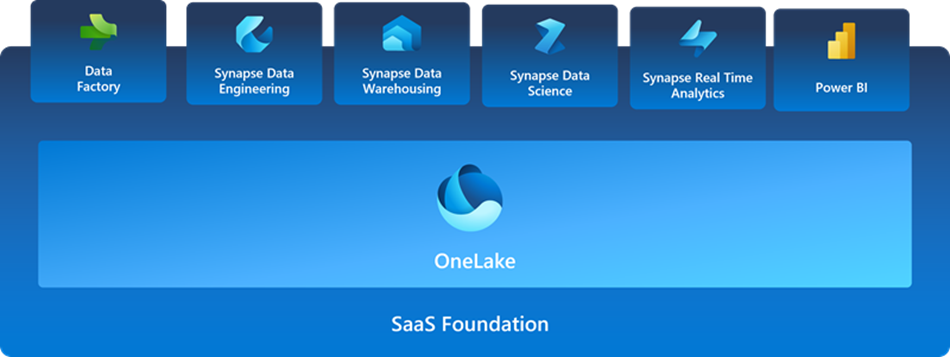
\includegraphics[width=12cm]{img/fabric.png}
  \end{center}
  \caption{Architektura platformy Microsoft Fabric \parencite{Buck2023}}
  \label{fig:fabric_architecture}
\end{figure}  

\paragraph{Jednotné datové úložiště Onelake}
Jedná se o základní stavební kámen platformy, který poskytuje jednotné datové úložiště typu Dala Lake. Služba OneLake má v rámci platformy Microsoft Fabric za úkol poskytovat jedinou datovou bázi, pro všechny procesy a výstupy z platformy. Tato centralizace pak přináší řadu výhod. Z hlediska samotných analytických dat se jedná zejména o udržování pouze jedné kopie dat a tím i jejich konzistence napříč všemi analytickými procesy a výstupy, dále je pak například značná výhoda v jednotném přístupu k datům, který je možný dle potřeby realizovat za pomocí analytického enginu Apache Spark, dotazovacího jazyků T-SQL a nebo KQL.\parencite{OneLake}

\paragraph{Data Factory}
Tato služba poskytuje škálovatelný nástroj, jehož účel je integrace a transformace dat. Primárně tedy slouží k poskytnutí tzv. ETL procesu, který je zodpovědný za extrakci, transformaci a nahrání dat k analytickému zpracování\footnote{Samotný proces je detailně  popsán v kapitole \ref{dwh}}. V rámci služby je možné vyfiltrovat potřebná data a poskytnout je dalším službám ke zpracování.\parencite{DataFactory}

\paragraph{Synapse Data Engineering}
Služba Data Engineering je určena pro návrh, tvorbu a údržbu potřebných infrastruktur, které umožňují sbírat, ukládat a zpracovávat velké objemy dat. Na rozdíl od služby Data Factory, je však navržena tak, že její výstupem je koncept jednotného datového úložiště Datalakehouse, který je možné pro tento účel vytvořit v rámci služby OneLake, dále pak služba samotná již poskytuje analytické nástroje a je hluboce integrována s analytickým enginem Apache Spark.\parencite{DataEngineering}

\paragraph{Synapse Data Warehousing}
Data Warehouse je služba, která má za cíl vytvoření datového skladu, pomocí který následně poskytuje rozhraní pro práci s uloženými daty za pomocí dotazovacího jazyka SQL. V rámci platformy Microsoft Fabric se tak děje pomocí tzv. virtuálního datového skladu postaveného na úložištěm OneLake, kterém jsou po zpracování data uložena ve formátu open Data Lake\footnote{viz. https://delta.io/} \parencite{DataWarehousing}

\paragraph{Synapse Data Science}
V rámci služby Data Science a jejímu propojení se službou Azure Machine Learning lze vytvářet modely určené pro strojové učení. Díky této službě je tak možné doplnit požadované výstupy o vylepšené predikce, kterých by bez strojového učení bylo komplikované dosáhnout.\parencite{DataScience}

\paragraph{Synapse Data Real Time Analytics}
Úkolem této služby je zpracování a analýza tzv. observačních dat, tedy dat, která jsou ve velkém objemu generována velkým množstvím zdrojů a která z principu ukazují aktuální stav sledované situace. Vzhledem k proměnlivým schématům a atypickým formátů bývají tato data komplikovaně zpracovatelná klasickým datovým úložištěm.\parencite{RealTimeAnalytics}

\paragraph{Power BI}
Power BI je služba jejímž primární účel je vizualizace zpracovaných dat. Primárním výstupem služby jsou interaktivní nástěnky, které je možné nasadit například ve formátu webové stránky a tím je velmi snadno zpřístupnit uživatelům.\parencite{PowerBi}\\

Za pomocí výše zmíněných komponent poskytuje platforma Microsoft Fabric velmi silný a univerzální nástroj, díky kterému je možné velmi efektivně vytvářet analytické nástroje a přehledy, které mohou čerpat data z velkého množství zdrojů, tato data následně integrovat, zanalyzovat a vyhodnotit. Díky integraci nástrojů určených pro strojové učení, umožňuje platforma i tvorbu pokročilých predikčních modelů.\\

Všechny výše zmíněné koncepty jednotných datových úložišť mají stále své opodstatnění a jsou stále hojně využívány. Volba správného typu úložiště vždy závisí na konkrétním případě pro které má být úložiště nasazeno, kdy například pro dlouhodobá statistická data je lepší úložiště typu Datový sklad, zatímco pro velké množství dat v reálném čase spíše využijeme Data Lake. Klesající náklady na provoz úložišť, však čím dál častěji umožňují firemní nasazení úložiště Data Lakehouse, které následně může sloužit jako primární datový bod pro celou organizaci a jehož data se dají následně dle potřeby analyzovat.


\chapter{Datový sklad}
\label{dwh}
Jak je uvedeno v předchozí kapitole, jednou z možností uložení dat je využití tzv. Datového skladu, který umožňuje jejich snadnou analýzu. Pojem datový sklad může mít vícero definic. Je možné na něj nahlížet například pouze jako na proces, který má zjednodušit přístup k datům a kdy je technické řešení datového skladu pouze podpůrný prvek celého procesu. Nejčastěji se však na datový sklad pohlíží jako na systém, který \emph{extrahuje, čistí, upravuje a dodává zdrojová data do dimenzionálního datového úložiště a poté podporuje a zavádí dotazování a analýzu dat za účelem rozhodování.} \parencite[s.~23]{Kimballc2004}

Z této definice jasně vyplývá, že primárním účelem datového skladu je centralizace a standardizace dat, díky které je pak přístup k datům značně usnadněn. Zároveň je zde důležité uvést, že každý datový sklad se skládá z několika komponent, z nichž pravděpodobně nejdůležitější je proces extrakce, čištění a úpravy dat. Tento proces se ve spojitosti s datovými sklady nazývá \emph{ETL proces \footnote{z angl. Extract, Transform and Load} }a je hlavním důvodem proč pojem datový sklad nelze zaměňovat s pouhým datový úložištěm. \parencite[s.~24]{Kimballc2004}

Využití datových skladů je pak velmi rozmanité, jednou z nejčastějších aplikací je ale jejich využití ve spojení se systémy podpory rozhodování \footnote{zkráceně DSS z angl. Decision support
systém}, kde často slouží jako primární znalostní báze. \parencite[s.~2]{Inmon2005}

Obecné schéma datového skladu je znázorněno na obrázku \ref{fig:dwh_schema}, na kterém je patrné, že primárním vstupem jsou data z různých zdrojů a typů. Jednotlivé druhy vstupních dat potřebují specifickou úpravu, za tím to účelem je zde již zmíněný ETL proces, který následně uloží zpracovaná data do datového skladu. Finálním výstupem jsou pak strukturovaná data, která typicky využívána pro business inteligence \footnote{zkráceně BI}, nebo jako přehledové dashboardy vizualizující provozní data, jako mohou být například přehledy spotřebovávané energie nebo obsazenosti kanceláři.

\begin{figure}[h]
  \begin{center}
          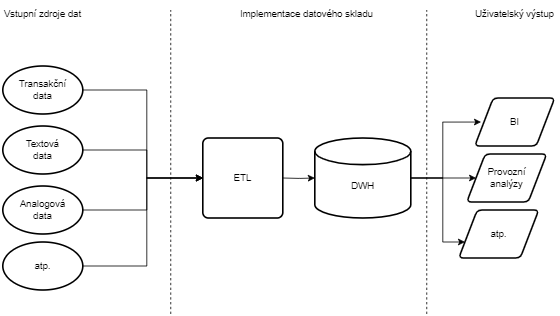
\includegraphics[width=12cm]{img/dwh_schma.png}
  \end{center}
  \caption{Obecné schéma datového skladu. Vlastní zpracování}
  \label{fig:dwh_schema}
\end{figure}  

\section{Typy datových skladů}
\label{dwh_types}
Datové sklady se dají rozdělit na několik druhů dle různých kritérií. \citeauthor{Inmon2005}
v knize \citetitle{Inmon2005} z roku \citeyear{Inmon2005} dělí datové sklady podle způsobu a rozsahu,
v jakém data shromažďují a dle prostředí, ve kterém je datový sklad nasazen.

Pro první rozdělovací kritérium, tedy dle rozsahu shromažďovaných dat zavádí Inmon postupně tři kategorie: hluboký datový sklad \footnote{angl. Deep Data Warehouse}, široký datový sklad \footnote{angl. Wide Data Warehouse} a hybridní datový sklad \footnote{angl. Hybrid Data Warehouse}. Tyto jednotlivé kategorie jsou pak definovány takto:
\paragraph{Hluboký datový sklad}
Shromažďovaná data jsou převážně historická a velmi detailní. Slouží primárně k analýze vývoje a trendů.
\paragraph{Široký datový sklad}
Zaměřuje se na velké spektrum informací, přičemž neukládá data v takovém detailu. Využívá se především pro tvorbu přehledů a rychlé vyhledávání dat.
\paragraph{Hybridní datový sklad}
Jedná se o kombinaci obou předchozích kategorií.

 \vspace{5mm}
Pokud datové sklady dělíme dle druhého kritéria, tedy dle prostředí, ve kterém je
nasazujeme, pak Inmon definuje čtyři kategorie, a to Operational Data Stores, Data marts,
Enterprise data warehouse a Virtual data warehouse. Tyto kategorie jsou pak dle Inmona definovány následovně:

\paragraph{Operational Data Stores}
Datový sklad, který je určen k provozním potřebám organizace, pro kterou je zřízen. Integruje a centralizuje data z firemních procesů.
\paragraph{Enterprise data warehouse}
Datový sklad, který centralizuje všechna data z celé organizace a slouží jako hlavní znalostní báze pro její řízení.
\paragraph{Data marts}
Malé datové sklady, typicky se budují pro jednotlivá oddělení organizací a na základě jejich specifických potřeb. Tento typ také někdy bývá realizován pouze jako podmnožina velkých datových skladů, jako je Operational Data Store nebo Enterprise data warehouse.\parencite{Inmon2021}
\paragraph{Virtual data warehouse}
Specifický typ datového skladu, který funguje pouze jako transportní a translační vrstva nad různými datovými zdroji a pro uživatele tak vytváří jeden přístupový bod. Data tedy nejsou uložena na jednom místě a ve strukturalizované podobě, ale jsou nahrávána z více externích zdrojů, následně dle potřeby přetransformovaná a doručena uživateli. 

\vspace{5mm}
Uvedené typy datových skladů je možné dále rozšířit o další poddruhy, jako je například koncept \emph{Data vault}, který se vyznačuje velmi vysokou mírou přesnosti dat a důslednou kontrolou jejich integrity, kdy je například uchovávaná i informace o jejich původu a je kladen velký důraz na jejich verifikaci a i následné využití. Tento typ datového sklad nachází uplatnění například v bankovním, armádním a nemocničním sektoru a z tohoto důvodu se většinou jedná o vysoce zabezpečené a neveřejné datové sklady.\parencite{Inmon2021}

Všechny zmíněné typy datových skladů vyžadují specifický přístup, a to jak
k architektuře samotného skladu, zpracování dat, tak i k technickému vybavení. Z tohoto
důvodu je důležité zvolit správný typ datového skladu již ve fázi návrhu, protože
možnost konverze mezi jednotlivými druhy datových skladů nemusí být vždy možná.

\subsubsection{Zpracování dat v datových skladech}
Vzhledem k tomu, že datový sklad většinou slouží jako koncentrátor dat z mnoha různých zdrojů, prochází data při nahrávání transformačním procesem, jehož výstupem jsou strukturovaná data. Celý tento proces bývá zpravidla automatický, byť to není nikterak podmíněno.

Proces nahrávání dat do datového skladu se nazývá ETL \footnote{z angl. Exract, Transform and Load} a jedná se o esenciální součást datového skladu. Celý proces se skládá, jak již název napovídá, ze tří fází, a to fáze extrakce, transformace a finálního nahrání dat do datového skladu.

Kimball a Caserta v knize \citetitle{Kimballc2004} z roku \citeyear{Kimballc2004} celý proces rozšiřují do fází čtyř, a to extrakce, čištění, potvrzovaní \footnote{angl. Conforming} a doručení. Vzhledem k tomu, že zmíněná publikace patří mezi základní v oboru datových skladů, budu se v další části zabývat jen tímto rozdělením ETL
procesu, a ne pouze základními třemi fázemi.

\subsection{ETL proces dle Kimballa a Casertyho}
\paragraph{Extract}
První operací, kterou je potřeba pro nahrání dat udělat, je jejich extrahování z původních úložišť. To probíhá většinou v přesně definovaných cyklech. Během této operace dojde k nahrání všech požadovaných dat do přechodného úložiště, kde jsou dále zpracovávány v dalších krocích ETL procesu. Data jsou nahrávána v surové formě a v původních formátech a souborech, které mohou představovat například data z relačních databází, XML, csv, JSON nebo XLS soubory.\parencite[s.~18]{Kimballc2004}

Surová data bývají po zpracování většinou smazána, výjimku tvoří například případy, kdy potřebujeme zachovat dlouhodobou zálohu dat, anebo pokud je potřeba porovnat změny dat mezi jednotlivými průběh extrakčních cyklů.\parencite[s.~18]{Kimballc2004}

V některých případech je možné využít jako zdroj dat pro datový sklad úložiště jiného typu, typicky například Data Lake.

\paragraph{Cleaning}
Poté, co jsou požadovaná data vyextrahována je potřeba je vyčistit. Během této fáze se provádí kontrola integrity dat, odstraňují se duplicity a provádějí další operace s cílem dosáhnutí požadované datové kvality.\parencite[s.~18-19]{Kimballc2004}

Během této fáze také dobré zvolit požadovanou granularitu dat, neboli míru detailu uchovávaných informací \parencite[s.~41]{Inmon2005}, a případně data na požadovanou úroveň zdecimovat. Granularita patří mezi základní parametry využívané při návrhu datového skladu, a tak by měla i její hodnota z tohoto návrhu vycházet.\parencite[s.~41]{Inmon2005}

\paragraph{Potvrzování (Conforming)}
Fáze potvrzování má význam zejména v případech, kdy extrahujeme data z více datových zdrojů. Jejím primárním úkolem je data z různých zdrojů propojit dohromady tak, aby bylo možné se dotazovat napříč všemi těmito zdroji. \parencite[s.~19]{Kimballc2004}

Dalším důležitým úkolem je pak kontrola konfliktů mezi názvy jednotlivých dimenzí, neboť napříč datovými zdroji nemusí mít vždy stejný význam. \parencite{Kimballc2004}

\paragraph{Doručení (Delivering)}
Během doručovací fáze dochází k samotné transformaci dat do jednotného formátu a následně se z dat vytvoří dimenzionální model, nebo požadované schéma. Mezi ty patří například schéma hvězdice či datová krychle.\parencite[s.~19]{Kimballc2004}

Výstupem této fáze je tedy patřičně setříděný a provázaný soubor dat, nad kterým je již možné provádět dotazy, jako nad celkem, tedy bez ohledu na datové zdroje a jejich formát. Takto zpracovaná data se pak následně nahrají do databáze samotného datového skladu.

Díky ETL procesu jsou ve výsledku v datovém skladu data uložena v jednoduché a snadno dovažovatelně formě, což značně usnadňuje a urychluje přístup a následnou práci s těmito daty.

\subsubsection{Využití datových skladů}
Datové sklady nacházejí velké využití zejména u velkých organizací a společností, ale i u tak velkých celků, jako jsou například samostatné státy. Velkou výhodou datových skladů je jejich perzistentní struktura, kdy data můžeme shromažďovat po dlouhou dobu a jejich analýzu provést až ve chvíli, kdy nastane její potřeba. Díky tomu se hodí na analýzu dat dlouhodobého charakteru.

Jedním z typických zástupců tohoto typu nasazení je pak sdílení dat mezi vědeckými pracovišti. Například v případové studii \citetitle{Seneviratne20180124} \parencite{Seneviratne20180124} se autoři zabývali propojením vědeckých pracovišť Stanford University, Stanford Cancer Institute a California Cancer Registry za účelem vytvoření společného datového skladu obsahujícího elektronické zdravotní záznamy pacientů postižených rakovinou prostaty. Díky tomuto datovému skladu vědci mají přístup k tisícům reálných případů, napříč těmito třemi institucemi.

Další zajímavou aplikací, je například optimalizace a analýza mléčné farmy. Tato aplikace popsaná v článku \citetitle{Schuetz20180326} \parencite{Schuetz20180326} se zabývá návrhem a implementací datového skladu, který má za cíl pomocí různých senzorů sledujících například pohyb dojnic či samotné dojení, optimalizovat a vylepšit výkon této mléčné farmy. Celý projekt je velmi zajímavý a to zejména z důvodu, že se jedná o specifickou oblast, kde ještě nebyl koncept datového skladu nasazen.

Zvláštním příkladem jednoúčelově zaměřeného datového skladu je projekt, týkající se pandemie viru SARS-COV-2. V článku \citetitle{Agapito2020} \parencite{Agapito2020}, autoři popisují implementaci datového skladu vytvořeného za účelem monitorování šíření viru v Itálii. Zajímavé je, že datový sklad zahrnuje kromě informací týkajících se přímo samotného viru i další, zdánlivě nesouvisející, informace, které zahrnují například také aktuálním stavu klimatu, jako je znečistěni ovzduší a nebo síla a směr větru. Výzkumné výstupy z tohoto projektu se tak mohou zabývat i vlivem počasí na šíření nákazy. 


Vzhledem k tomu, že datové sklady typicky zpracovávají a následně drží velké množství dat, je zbytečné, poskytovat všechna data všem uživatelům, z tohoto je běžné, že na základě velkým datový skladů vznikají malé specializované sklady tzv. \emph{data marts} viz. \ref{dwh_types}, které využívají datovou bázi \emph{mateřského} datového skladu a následně poskytují pouze přesně zacílené informace, které jsou relevantní pro dané uživatele, typicky firemní oddělení, čímž došlo ke vzniku tzv. \emph{the corporate information factory}.\parencite{Inmon2021} Tento koncept je znázorněn na obrázku \ref{fig:data_marts_schema}, ze kterého je zřejmé, že pro chod celé informační infrastruktury je využíváno více datových skladů, na jejichž základě jsou pak vytvářeny jednotlivé specializované sklady.

\begin{figure}[h]
  \begin{center}
          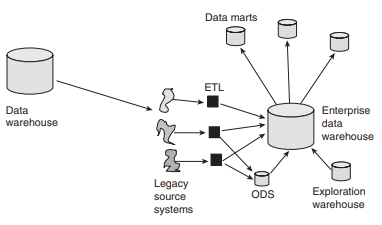
\includegraphics[width=10cm]{img/data_marts_schema.png}
  \end{center}
  \caption{Korporátní informační struktura \parencite[s.12]{Inmon2008}}
  \label{fig:data_marts_schema}
\end{figure}  



\chapter{ITSM}
Jak již bylo zmíněno v úvodní kapitole, velký rozmach informačních technologií a služeb v 60. letech 20. století si vyžádal vznik patřičných standardizovaných procesů, postupů a pravidel pro řízení služeb v prostředí podniků a organizací. Souhrnně je tento obor označován jako ITSM, neboli Information Technology Service Management, což je pojem, který se původně objevil pouze v rámci metodiky ITIL, ale postupně se rozšířil a zobecnil tak, že v současné době obecně pokrývá problematiku řízení IT služeb.\parencite[s.~20]{Matula2017} 

Matula definuje ITSM jako \textit{souhrn nejlepších praxí a referenčních modelů procesů řízení služeb IT organizace}, přičemž právě přístup, kdy se k IT projektu přistupuje jako k službě znamená, že se daný IT projekt dodává s potřebným personálním a technologickým zajištěním a samotný klient se na chodu dané služby nepodílí a využívá pouze její výstupy.\parencite[s.~20-22]{Matula2017}

\section{Základní terminologie ITSM}
Před samotným zavedením a ukotvením základních principů fungování ITSM je nutné nejprve zavést alespoň základní pojmy, které jsou v jeho rámci využívány. Matula ve své publikaci \citetitle{Matula2017} uvádí jako základní tyto následující pojmy, jejichž definice jsou převzaty z \citetitle{SyFvQA11lk1OaIec} z roku \citeyear{SyFvQA11lk1OaIec}:
\paragraph{Nejlepší praktiky (Best practices)}
Osvědčené postupy, které byly využívány ve více organizacích a které se prokázaly jako účinné, efektivní a udržitelné a které vedou k zlepšení výsledků v oblasti kvality, flexibility, nákladů a konkurenceschopnosti.
\paragraph{Služba (Service)}
Prostředek, který zajišťuje doručování hodnoty zákazníkovi, bez nutnosti zapojení zákazníka do řízení nákladů a rizik. Pojem služba může být chápán několika způsoby a to buď jako obecná služba, IT služba, anebo balíček několika služeb. 
\paragraph{Správa (Governance)}
Zajišťuje, aby byly procesy vykonávány správně dle nastavených politik a strategií. Správa zároveň vymezuje role a odpovědnosti, reaguje na zjištěné problémy.
\paragraph{Proces (Process)}
Soubor aktivit, které je třeba vykonat pro dosažení cíle. Aktivity přijímají definované vstupy, které následně za pomoci nástrojů transformují na požadované výstupy.
\paragraph{Funkce (Function)}
Pojem funkce má několik významů. Primárně se jedná o skupinu lidí, nástrojů a jiných zdrojů, které zainteresované osoby využívají k provádění procesů a činností. Dále se pak může jednat o zamýšlený účel konfigurační položky, osoby, týmu nebo procesu. Posledním významem pojmu je pak vyjádření toho, zda je zamýšlený úkol vykonáván správně. 
\paragraph{Role (Role)}
Soubor činností, povinností a pravomocí přidělených konkrétní osobě, anebo skupině osob. Jednotlivec, nebo skupina může mít více rolí.
\paragraph{Kvalita (Quality)}
Schopnost služby, výrobku nebo procesu poskytnout požadovanou hodnotu. Kvalita je ukazatel účinnosti a efektivity procesů.
\section{Základní principy ITSM}
V úvodu této kapitoly již byly využity termíny, jako je proces a nebo kvalita výstupu, které patří do základní terminologie ITSM, a které je potřeba nejdříve definovat. Zde uvedené definice vychází zejména z frameworků, které jsou na ITSM postaveny

Management IT služeb se dle ITSM věnuje několika oblastem, které ovlivňují výslednou kvalitu výstupu a které jsou:
\begin{compactitem}
  \item Lidé, což je oblast zahrnující veškeré lidské zdroje, které jsou potřeba k implementaci a provozu samotné služby, přičemž zahrnuje i uživatele, kteří službu využívají.
  \item Procesy, což je oblast zahrnující veškerou procesní metodiku a postupy, které jsou využívány k řízení a implementaci služeb a to včetně jejich vstupů, výstupů a zodpovědných osob.
  \item Nástroje, které zahrnují veškeré softwarové i hardwarové vybavení, které umožňuje dané procesy zefektivnit či zautomatizovat.
\end{compactitem}

V rámci poskytování služeb je také důležité hlídat kvalitu výstupů. Za tímto účelem definuje ITSM základní indikátory, které umožňují kvalitu služby měřit a následně vyhodnotit. Konkrétně se pak jedná o tyto složky IT služeb \parencite[s.~20]{Matula2017}:
\begin{compactitem}
\item Růst a hodnota jsou ukazatele, které se zabývají změnou výnosů před a po zavedení dané služby.
\item Rozpočet a jeho dodržování, jakožto ukazatelů zabývajících se optimalizací projektového rozpočtu s cílem eliminovat zbytečné výdaje.
\item Riziko dopadu, které indikuje a vyhodnocuje následky případných rizik.
\item Efektivita a komunikace, vyhodnocující zpětnou vazbu od zákazníků a jejich spokojenost s poskytovanými službami.
\end{compactitem}

ITSM je v současnosti popsán normou ISO 20000 Informační technologie - Management služeb IT a na jejímž základě existuje mnoho různých frameworků a knihoven nejlepších praktik. Patří mezi ně například COBIT, FitSM a zejména pak ITIL.\parencite[s.~25]{Matula2017}

\begin{figure}[h]
  \begin{center}
          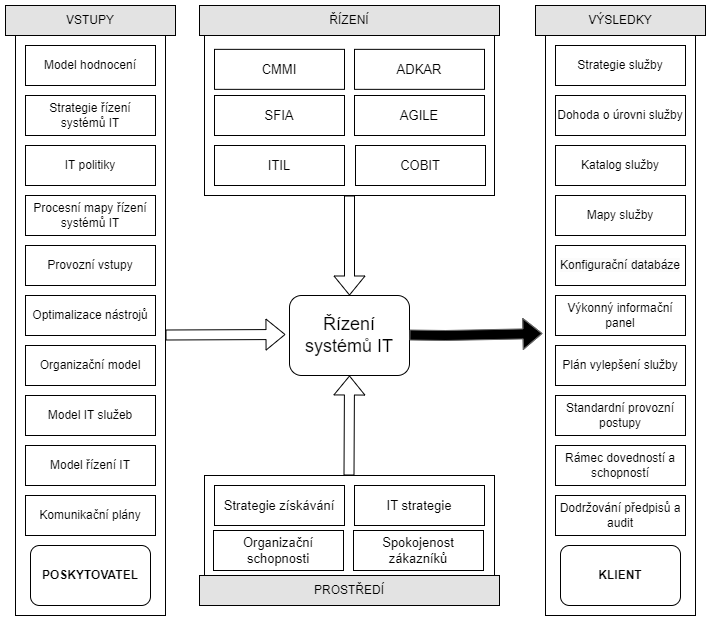
\includegraphics[width=10cm]{img/itsm-diag.drawio.png}
  \end{center}
  \caption{Řízení systémů IT \parencite[s.~21]{Matula2017}}
  \label{fig:itsmDiag}
\end{figure} 

Souhrnné schéma ITSM je vyobrazené na obrázku \ref{fig:itsmDiag}, ze kterého je patrné, že samotné ITSM je postaveno na čtyřech pilířích. Základní dvojici tvoří vstupy a výsledky. Díky vstupům může poskytovatel dodat zákazníkovi potřebné výsledky, neboli hodnotu. Tento proces je pak ovlivňován prostředím, ve kterém je služba realizována a které do značné míry ovlivňuje způsob realizace. Poslední částí je pak řízení, které určuje metodiku, kterou je služba realizována. 


\section{ITIL}
Jednou z nejrozšířenějších knihoven v oblasti ITSM je knihovna ITIL \footnote{z angl. Information Technology Infrastructure Library}, která je v současnosti spravována britskou společností Axelos Ltd. \parencite[s.~31]{Matula2017}. Tato knihovna byla dle průzkumu Forbes Insight z roku 2017 částečně implementována alespoň ve 47\% zkoumaných organizací\parencite{Watts3082017} a byla využita i při  zavádění datového skladu na Masarykově univerzitě. 

ITIL vznikl v 80. letech 20. století na objednávku britské vlády a původně byl nazýván GITIM \footnote{z angl. Government Information Technology Infrastructure}. Během 90. let byl dobře přijímán velkými organizacemi a vládami, což z něj učinilo standard na poli ITSM knihoven a frameworků, a i nadále slouží jako základ pro nové frameworky, které jsou z něj odvozeny, jako je například MOF\footnote{z angl. Microsoft Operations Framework} od společnosti Microsoft. \parencite[s. ~31]{Matula2017}

Knihovna ITIL je průběžně aktualizována a momentálně nejrozšířenější jsou verze 3 z roku 2007 a verze V4 z roku 2017. Mezi těmito verzemi došlo k velké změně pojetí. 

Třetí verze frameworku se ITIL se věnuje převážně samotnému procesu zavádění služby, od jejího návrhu, přes realizaci, až po každodenní využití služby. Jejím základním cílem je optimalizace procesů IT oddělení společností a organizací tak, aby byly v souladu s jejich obchodními cíli. Primárně má za úkol zajistit, aby byly realizované služby řízeny právě obchodními požadavky a samotné IT oddělení má za cíl pouze jejich implementaci.\parencite[s.~8]{Carlidge2007} Oproti tomu ITIL ve verzi V4 se primárně věnuje doručované kvalitě, nákladům a rizikům. 

Zjednodušeně řečeno ITIL ve verzi 3 cílí na fungování dodavatele, coby pouhého realizátora služby a na proces vedoucí k jejímu poskytování. Oproti tomu ITIL verzi 4 se zaobírá především důvody a cíli, které ke vzniku služby vedly.\footnote{https://www.alvao.com/cs/blog/dlouha-cesta-k-itil4-jak-nam-historie-itil-pomuze-lepe-ridit-it se pak rozhodni jestli to chceš ocitovat a jak}
Z důvodu této velké  odlišnosti jsou obě verze detailně popsány v následujících kapitolách.  
\subsection{ITIL V3/ITIL 2011}
Jak již bylo uvedeno v předchozí kapitole, knihovna ITIL ve verzi 3 byla představena v roce 2007. V roce 2011 však prošla aktualizací a bývá tak označována jako ITIL 2011. Aktualizace se týkala především zavedení nových procesů a prohloubení definic stávajících procesů a pojmů. Nicméně i přes tuto aktualizaci zůstávají verze V3 a 2011 kompatibilní.\parencite{Kempter2722013}

Jak je znázorněno na obrázku \ref{fig:itil3_lifecycle}, knihovna ITIL 2011 se věnuje celistvému procesu managementu služeb, od stanovení obchodní strategie, přes její vývoj a nasazení do provozu až po kontinuální vylepšování. 
  
\begin{figure}[h]
  \begin{center}
          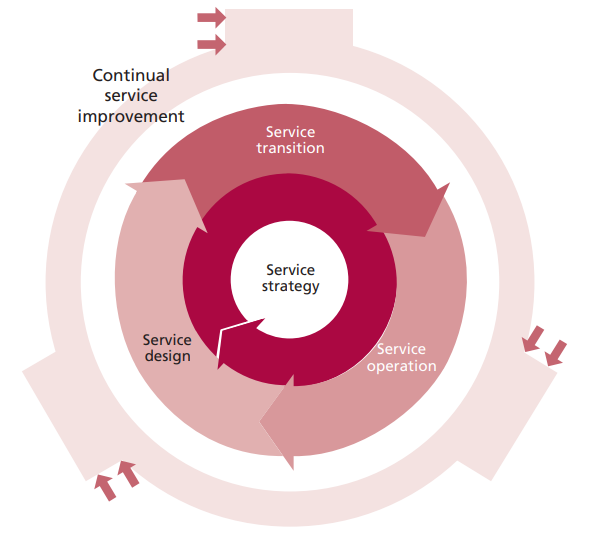
\includegraphics[width=10cm]{img/itil_V3_proces.png}
  \end{center}
  \caption{Životní cyklus ITIL 2011 \parencite[s.~7]{Carlidge2007}}
  \label{fig:itil3_lifecycle}
\end{figure}  

Na obrázku \ref{fig:itil3_schema} je znázorněno schéma celé knihovny ITIL 2011, která je členěna na pět fází, které se postupně věnují celému procesu managementu služeb - od obchodní analýzy a strategie, přes její design, nasazení a správu až po její následný rozvoj. Ze schématu je také patrné, že fáze se skládají z jednotlivých procesů a funkcí, které slouží k samotné realizaci.

\begin{figure}[h]
  \begin{center}
          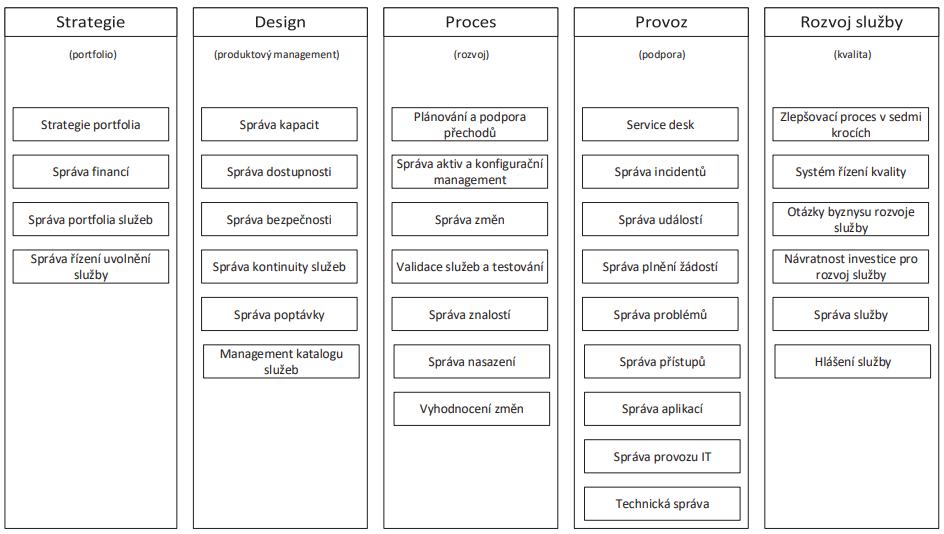
\includegraphics[width=11cm]{img/itil_V3_schema.png}
  \end{center}
  \caption{Schéma ITIL 2011 \parencite[s.~32]{Matula2017}}
  \label{fig:itil3_schema}
\end{figure} 


Každá fáze, která je vyobrazena na obrázku \ref{fig:itil3_schema} je v knihovně ITIL 2011 zastoupena samostatnou publikací. Ta problematiku dané fáze do detailu rozebírá a popisuje jednotlivé procesy a funkce. V rámci knihovny ITIL 2011 je zastoupena samostatnou publikací. 
\paragraph{Strategie služeb}
První publikace se zabývá návrhem strategie nové služby tak, aby primárně řešila daný obchodní problém s důrazem na kvalitu výstupu. Tato kvalita musí vycházet z požadavků klienta, pro kterého je služba navrhována a poskytována, ale zároveň musí nové služby být plně kompatibilní s interními procesy jak poskytovatele služby, tak i s procesy samotného klienta.\parencite[s.~12-13]{Carlidge2007}

Pro nastavení kvalitní strategie služby je nutné správně určit odpovědi na několik základních otázek, které následně slouží jako základní parametry pro vznikající strategii.\parencite[s.~32]{Matula2017} Mezi tyto základní otázky patří například následující:

\begin{compactitem}
  \item Jaké služby nabízet
  \item Kdo je jejich možný odběratel
  \item Co je hlavní doručovanou kvalitou realizované služby
  \item Jakým způsobem budou služby finančně řízeny a kontrolovány
  \item Metodika určování možných vylepšení služby a jejich prioritizace
  \item Jak robustní má služba být, aby byly dostatečně ochráněny investované zdroje a manažerské kapacity
  \item Jakým způsobem se bude měřit efektivita a výkon dané služby
\end{compactitem}

Po zodpovězení těchto základních otázek, je následně při návrhu služeb nutné dodržet princip tzv. čtyř P, který je realizován pomocí následující bodů:\parencite[s.~13]{Carlidge2007}
\begin{compactitem}
    \item Perspektiva - určuje charakteristické vize a směr dané strategie
    \item Pozice - udává základ, ze kterého má poskytovatel služby vycházet
    \item Plán - říká jakým způsobem má být daných cílů dosaženo
    \item Předloha - určuje základní postup rozhodování a realizace jednotlivých kroků a řešení problémů
\end{compactitem}

Kvalitní zpracování konceptu čtyř P zaručuje, dostatečně kvalitní základ pro další fáze managementu služeb.


\paragraph{Design služeb}
Druhá publikace se zabývá metodikami návrhu a změn samotných služeb, a to tak aby byla zajištěna správná funkcionalita služby s ohledem na požadované obchodní cíle a jejich případnou změnu. Za tímto účelem poskytuje publikace dva základní postupy. Prvním je správné vedení designu, vývoje služeb a praktik určených k jejich managementu. Druhým jsou pak základní metody a principy konverze strategických cílů v samotné službě.\parencite[s.~21]{Carlidge2007}

Za tímto účelem publikace definuje několik aspektů a principů. Prvním z nich je petice základních aspektů designu služeb, které jsou: \parencite[s.~22]{Carlidge2007}
\begin{compactitem}
    \item Řešení nově vznikajících a měnících se služeb
    \item Management informačních systémů a nástrojů
    \item Technologie a architektura managementu služby
    \item Procesy stanovené v rámci poskytování služby
    \item Měřící metriky a metody
\end{compactitem}
Pomocí těchto klíčových aspektů je zaručen holistický přístup a konzistence navrhovaných služeb v rámci organizace a správná integrace procesu v rámci IT oddělení a celé organizace, která dané služby poskytuje. \parencite[s.~22]{Carlidge2007}

Druhým klíčovým principem jsou čtyři P designu služeb, jejichž cílem je zajistit dobrou efektivitu služeb. Mezi tyto klíčové body patří:\parencite[s.~22]{Carlidge2007}

\begin{compactitem}
    \item Lidé (People), kteří jsou zainteresování v poskytování dané služby
    \item Produkty které zastupují technologie a spravované systémy, které slouží k doručení služby
    \item Procesy, role a aktivity, které slouží k poskytování služby
    \item Partneři, kteří zastupují dodavatele, výrobce a prodejce, kteří zajišťují dané službě podporu
\end{compactitem}

Posledním základním principem, které jsou v publikaci definovány je  \emph{Balíček designu služeb \footnote{z angl. Service Design Package, zkráceně SDP}}, který na základě dříve zmíněných hledisek a principů, definuje všechny aspekty služby a požadavků na ni v každé fázi jejího životního cyklu. SDP je vytvářeno s každou novou IT službou, aktualizací a nebo ukončením jejího poskytování.\parencite[s.~23]{Carlidge2007}
\paragraph{Přechod služeb}
Obsahem třetího svazku je popis správné metodiky, která má za úkol zajistit doručení nových a upravených služeb a služeb, u kterých bylo poskytování již ukončeno, a to s ohledem na naplněni obchodních cílů vycházeních ze strategie a designu služeb ustanovených dle první a druhé publikace.\parencite[s.~30]{Carlidge2007}

Klíčovým prvkem této fáze životního cyklu služeb je tedy nastavení správných manažerských procesů, které se zabývají nasazením služby do provozu, rizikového managementu, nastavení očekávaných výstupů, testování, přenosu znalostí týkajících se služeb atp.\parencite[s.~30]{Carlidge2007}

V rámci přechodu služby je nutné zadefinovat základní parametry, které umožňují službu správně zrealizovat. Tyto jsou zastoupeny následujícími body:\parencite[s.~30]{Carlidge2007}
\begin{compactitem}
    \item Potenciální obchodní hodnota, kdo jí doručuje a vyhodnocuje
    \item Identifikace všech zainteresovaných osob, které mají na úspěšný přechod vliv
    \item Implementace a případná adaptace designu služby, pokud se během přechodu ukáže nutnost změn
\end{compactitem}

Na základě těchto tří parametrů je následně možné realizovat přechod, který stojí na následujících základních principech, které zaručují efektivní efektivní přenos nové nebo modifikované služby. \parencite[s.~30]{Carlidge2007}
\begin{compactitem}
    \item Správné pochopení všech aspektů, principů, záruk a výstupů podpory služby
    \item Dobře zmapovaná komplexita technologických změna  procesů služby
    \item Ustavení manažerského rámce zavádění změn za účelem zajištění správného doručení výstupů a zvážení všech rizik
    \item Podpora přenosu znalostí a rozhodovacích kritérií týkající se všech procesů a funkcí služby a jejich správný přenos mezi všemi zainteresovanými stranami
    \item Ustanovení procesů které mají za úkol předvídat potřebné změny a jejich správné načasování
    \item zajištění zapojení veškerých stran zapojených do přechodu služby a jejich zaškolení do všech aspektů týkajících se přechodu služby
\end{compactitem}

Přenos služby spravovaný dle těchto pravidel zajišťuje bezproblémové uvádění nových a modifikovaný služeb do provozu a stejně tak i jejich ukončení. 
\paragraph{Správa služeb}
Čtvrtou fází životního cyklu služby dle ITIL 2011 je správa provozu samotné služby a jejím primárním cílem je zajištění, že služba bude doručovat nasmlouvanou hodnotu v požadované kvalitě.\parencite[s.~36]{Matula2017}

Tato fáze je oproti předchozím mírně specifická, a to jednak tím, že se prakticky výhradně zabývá uživateli služby a dále pak tím, že kromě procesů jsou v rámci této publikace definovány čtyři základní funkce, které je nutné v rámci správné implementace správy služeb dle ITIL 2011, zavést. Tyto základní funkce jsou: \parencite[s.~46]{Carlidge2007}
\begin{compactitem}
    \item Service desk - poskytuje uživatelům jednotný kontaktní bod, přes který je možné zaznamenávat změnové požadavky, incidenty, přístupové požadavky atp. 
    \item Technický management - umožňuje management správců technické infrastruktury, který pomáhá plánovat, implementovat a u udržovat stabilní technické prostředí pro správné fungování služby.
    \item Aplikační management - zajišťuje správu všech aplikací, které služba využívá, často je tato funkce využívána napříč různými službami, neboť samotné aplikace mohou být využívaný více službami.
    \item Řízení provozu IT - spravuje IT infrastrukturu služeb. Výše zmíněný technický management se nevěnuje primárně IT infrastruktuře, nýbrž obecně technickému zajištění služby. Tato funkce má zadefinovány také dvě podružné funkce, které se věnují personálnímu zajištění a správě fyzických zařízení, jako jsou typicky například data centra.
\end{compactitem}

\paragraph{Průbežné zlepšování služby}
Pátý a poslední svazek se zabývá průběžným vylepšováním služeb tak, aby byla vždy doručená požadovaná hodnota, která se může v průběhu času měnit. Vzhledem k tomu, že tyto změny probíhají na již fungující službě, je v rámci jejich návrhu, vývoje a nasazení využíván mechanismus PDCA\footnote{Zkratka prvních písmen anglických slov Plan, Do, Check a Act} neboli Demingův cyklus. Ten proces zavádění průběžných změn dělí do čtyřech následujících fází: \parencite[s.~38]{Matula2017}
\begin{compactitem}
    \item Plánuj - Určení strategie, která má vést k zlepšení a definování potřebných metrik
    \item Dělej - Sběr a zpracovaní potřebných dat
    \item Kontroluj - Analýza nasbíraných informací a údajů, jejich prezentace a využití
    \item Jednej - Aplikace vylepšení dané služby
\end{compactitem}
Mechanismus PDCA tímto zajišťuje, že je služba neustále hodnocena z hlediska doručované hodnoty a její kvality, čímž je zajištěn její postupný vývoj po malých krocích, jejichž realizace typicky bývá méně náročná i riziková. 

Tyto publikace dohromady tvoří základní korpus samostatné knihovny a jsou dále doplněny dalšími publikacemi a informačními zdroji, které se dané problematice věnují více do hloubky. \parencite[s.~8]{Carlidge2007}

\subsection{ITIL V4}
Nejnovější verze frameworku ITIL, tedy verze 4, byla uvedena v roce 2019. Jak již bylo uvedeno úvodu kapitoly, mezi verzemi V3 respektive 2011 a verzí 4 došlo k velmi výrazným změnám. Čtvrtá verze knihovny ITIL je oproti svým předchůdcům založena velmi holisticky a její primárním zaměřením není samotný proces, kterým je služba realizována a poskytována, ale zaměřuje se primárně doručenou hodnotu a její kvalitu a to zejména z hlediska uživatele uživatele služeb. Tato verze knihovny již také implementuje moderní metody vývoje, jako je Lean, Agile a nebo DevOps, které již nativně pracují s kontinuálním vylepšováním služeb. \parencite[s.~7]{Cartlidge2020}

ITIL V4 na rozdíl od předchozí verze nepracuje s jednotlivými fázemi realizace služby a místo toho zavádí nový koncept zvaný \emph{Service Value System}\footnote{zkráceně SVS}, který se skládá ze čtyř vrstev, které jsou definovány v další části této kapitoly. SVS vychází ze čtyři základních dimenzí managementu služeb, jejichž schéma je zobrazeno na obrázku \ref{fig:itil4_dimension}. Tyto základní dimenze poskytují holistický přístup k celému managementu služeb a ovlivňují všechny aspekty SVS.\parencite[s.~10]{Cartlidge2020} Definice jednotlivých dimenzí je pak následovná:

\begin{figure}[h]
  \begin{center}
          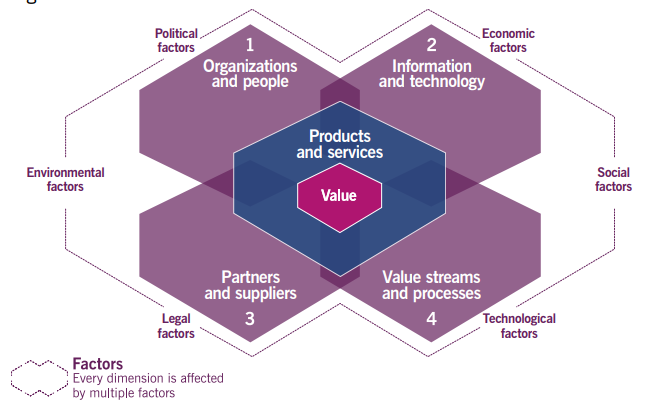
\includegraphics[width=11cm]{img/ITIL_V4_dimesions.png}
  \end{center}
  \caption{Čtyři základní dimenze managementu služeb \parencite[s.~32]{Cartlidge2020}}
  \label{fig:itil4_dimension}
\end{figure} 

\begin{compactitem}
    \item Organizace a lidé (Organizations and people) - První dimenze se věnuje primárně samotné správě organizace a vnitřní struktuře jejího personálního zajištění, dále může zahrnovat i samotné zákazníky a odběratele služeb a další zainteresované osoby nebo dodavatele. Všechny takto zainteresované strany musí být začleněny do jasné hierarchie, která reflektuje jejich schopnosti a cíle. 
    \item Informace a technologie (Information and technologies) - Tato dimenze se věnuje informacím a znalostem, které jsou potřeba k úspěšnému poskytovaní služby. Informace a znalosti jsou shromažďovány s ohledem a s důrazem na technologie, které jsou využívány v rámci správy služeb. Mezi takto spravované zdroje tak patří například databáze, komunikační systémy, cloudová prostředí, ale i například vytvořená, spravovaná a archivovaná data.
    \item Partneři a dodavatelé (Partners and suppliers) - V rámci třetí dimenze jsou řešeny vztahy mezi partnery a dodavateli, na kterých bývá realizace většiny služeb závislá, jelikož málo kdy jsou služby absolutně nezávislé na externích subjektech. V rámci těchto externích subjektů je nutné definovat hloubku propojení a integrace mezi nimi. Klíčovými faktory je pak správná kooperace těchto subjektů a to z hlediska nákladů, sdílení vědomostí a požadavků.
    \item Hodnotové proudy a procesy (Value streams and processes) - Čtvrtá dimenze definuje činnosti, pracovní postupy, procesy a jejich kontrolu tak, aby došlo k dosažení požadovaných cílů. Primárním oborem zájmu je tak v tomto případě hlavně zajištění komunikace a kolaborace mezi jednotlivými částmi organizace, která má za úkol poskytování dané služby, dále se pak dimenze zabývá tzv. hodnotovým tokem, který je definován jako \emph{řada kroků, které je třeba vykonat aby došlo k vytvoření a dodání požadované hodnoty klientům.}
\end{compactitem}
    
Mimo tyto hlavní dimenze je, vzhledem k tomu, že služby nejsou provozovány v uzavřeném prostředí, nutné zohlednit i externí faktory, které samotný design, vývoj i provoz ovlivňují a které se v určitém ohledu dají brát jako jedna ze základních dimenzí, jelikož je nikdy není možné úplně vyloučit. Na schématu \ref{fig:itil4_dimension} jsou vyznačeny jako vnější obálka zahrnující politické, ekonomické, sociální, technologické, právní a enviromentální faktory, zkráceně se pro tyto faktory používá zkratka PESTLE.\footnote{z angl. Political, Economic, Social, Technological, Legal and Enviroment}

\vspace{5}
Jak již bylo zmíněno, tak na výše definovaných základních dimenzích je postaven nový systém správy služeb, který se nazývá Service Value System, neboli SVS. Tento systém se skládá z několika vrstev, jejichž schéma je znázorněno na obrázku \ref{fig:SVS_schema}. Ze schématu vyplývá, že prvotními vstupy jsou požadavky nebo příležitosti, které postupně procházejí jednotlivými vrstvami přes hlavní principy managementu služby, její správu, řídící postupy až po průběžné vylepšení, ústřední části je pak \emph{Service value chain}. Na konci toho procesu je výstupem hodnota v požadované kvalitě. \parencite[s.~14]{Cartlidge2020} Významy a obsah jednotlivých vrstev, je detailně rozepsán níže. 
    \begin{figure}[h]
        \begin{center}
            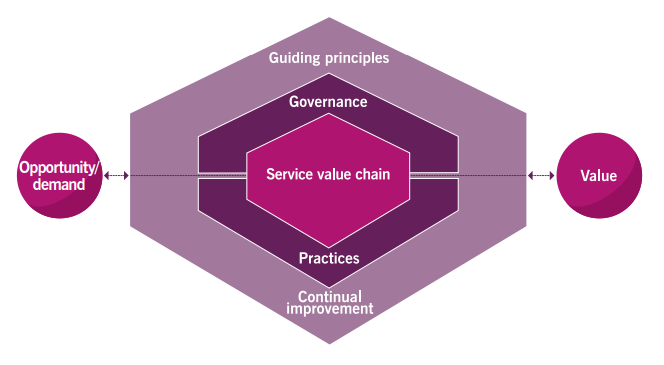
\includegraphics[width=11cm]{img/SVS_schmea.png}
        \end{center}
        \caption{Schéma SVS \parencite[s.~21]{Cartlidge2020}}
        \label{fig:SVS_schema}
    \end{figure} 

\begin{compactitem}
    \item Hlavní principy (Guiding principles) - První vrstva se zabývá komplexním řízením celé organizace a za všech situací a vytváří základy pro interní kulturu poskytovatele, rozhodovací mechanismy a celkově proces pro řízení poskytování služeb. Tato vrstva je rozdělena na sedm klíčových principů, které pokrývají celý proces poskytování služeb. 
    \begin{compactitem}
      \item Zaměř se na hodnotu - Nejdůležitější je doručená hodnota a její kvalita, ať pro uživatele služby, tak pro samotného dodavatele. Důležitým ukazatelem kvality služby je v tomto případě tzv. Customer Experience\footnote{zkráceně CX}, který udává jak je uživatel s danou službou spokojený.
      \item Začínej v aktuální situaci - není nutné vždy začít vyvíjet službu od začátku, je vhodné stavět na již existujících prostředcích, službách atp., neboť vývoj od samého začátku je velmi náročný na zdroje a z pravidla zahrnuje i již jednou řešené situace. 
      \item Postupuj iterativně a s ohledem na odezvu - Velké úkoly je nutné rozdělit do menších celků, které se dají lépe spravovat a řídit a to jednak v ohledech kontroly jejich samotné realizace, tak s ohledem na snazší řešení případných problémů. Jednotlivé úkoly by měly být zaváděny postupně a s ohledem na odezvu, neboť se v průběhu vývoje či poskytování mohou požadavky na službu lišit. 
      \item Collaborate and promote visibility - Personál musí spolupracovat a zajišťovat, aby každý, kdo je zainteresovaný do procesu poskytování služby, měl přiřazenou patřičnou roli, která odpovídá jeho schopnostem. Je důležité, aby byla pracovní náplň jednotlivců či týmů známá, neboť je tak možné snáze hledat chyby a případně změny v projektu a zjednat jejich nápravu.
      \item Mysli a pracuj holisticky - Žádný ze zdrojů potřebných pro realizace a poskytování služby není od ostatních izolován a nejedná samostatně. Cílem je, aby v celém procesu nevznikala slepá a neznámá místa, celý proces musí přesně zmapován od požadavku do doručení kvality.
      \item Udrž to jednoduché a praktické - Cílem je využívat co nejjednodušší postupy a zdroje. Je důležité uchovávat v provozu pouze ty zdroje, procesy, metriky atp., které přinášejí požadovaný výstup. 
      \item Optimalizuj a automatizuj - V rámci organizace je důležité automatizovat rutinní úkoly v co největší míře, což vede k úspoře nákladů a zpravidla i k menší chybovosti. Zautomatizované úkoly je nutné udržovat v optimalizované formě, neboť neoptimalizované procesy mohou naopak organizaci zatěžovat.
    \end{compactitem} 
    \item Správa (Governance) - Druhá vrstva se věnuje nastavení potřebných procesů pro řízení a reporting uvnitř organizace poskytující služby. Může se jednat o celou organizaci a nebo jen její dílčí části, cílem je zajištění správného směřování vůči cílům a prioritám organizace. 
    \item Hodnotový řetězec služby - Jak již bylo zmíněno výše, jedná se o soubor kroků, které je třeba provést, aby z dodaných vstupů vznikla požadovaná hodnota. Tento řetězec se skládá z šesti samostatných aktivit a celé schéma hodnotového řetězce je vyobrazeno na obrázku \ref{fig:value_chain}, jeho jednotlivé části jsou pak definovány následovně:
    \begin{compactitem}
        \item Plan - Zajišťuje sdílení jednotné vize, stavu a směru dalšího vývoje produktu či služby.
        \item Zlepšení - Věnuje se postupnému zlepšování služby, nebo produktu.
        \item Zapojení - Zajišťuje správné pochopení potřeb všech zainteresovaných stran, jejich transparentnost a kontinuální zapojení. 
        \item Design a přechod - Zprostředkovává kontrolu kvality výsledného produktu/služby, nákladů a jejich uvedení na trh.
        \item Získávání/budování - Zabezpečuje, že jsou jednotlivé komponenty služby/produktu dostupné, když jsou potřeba a dle potřebných specifikací.
        \item Doručení a podpora - Zaručuje doručení produktu/služby dle domluvených specifikací a očekávání zainteresovaných stran.
    \end{compactitem}
    Hodnotový řetězec služby je značně flexibilní a umožňuje nasazení v rámci nejrůznějších vývojových přístupů. Díky této flexibilitě umožňuje velmi snadno, rychle a efektivně reagovat na případné změnové požadavky zainteresovaných stran. Spolu s praktikami ITIL tak tvoří velmi komplexní sadu nástrojů pro správu IT služeb.\parencite[s.~21]{Cartlidge2020}

    \begin{figure}[h]
        \begin{center}
            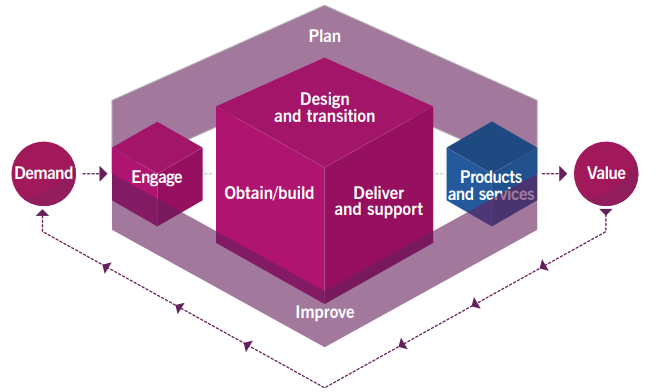
\includegraphics[width=11cm]{img/value_chain.png}
        \end{center}
        \caption{Service Value Chain \parencite[s.~21]{Cartlidge2020}}
        \label{fig:value_chain}
    \end{figure} 
    
    \item Postupy (Practices) - V rámci třetí vrstvy je definována řada postupů, které jsou designovány dle čtyř základních dimenzí managementu služeb a každá podporuje více hodnotových řetězců. Tyto postupy se dělí do tří kategorií a to \emph{Obecné manažerské postupy}, \emph{Postupy managementu služeb} a \emph{Postupy technického managementu}, jejich kompletní seznam je pak uveden v tabulce \ref{tab:management_practices_ITIL}.
    Tyto postupy jsou navrženy tak, aby zajistili správné pochopení a ukotvení celkového přehledu tykajícího se struktury, obsahu a klíčových konceptů uživateli služby nebo produktu. Z tohoto jsou všechny vystavěny dle následujícího schématu: \parencite[s.~23]{Cartlidge2020}
    \begin{compactitem}
        \item Obecné informace
        \begin{compactitem}
            \item Účel a popis
            \item Termíny a pojmy
            \item Rozsah/záběr
            \item Faktory úspěšné praxe
            \item Klíčové metriky
        \end{compactitem}
        \item Hodnotové proudy a procesy
        \begin{compactitem}
            \item Jak praxe přispívá k činnostem hodnotového řetězce služeb
            \item Procesy a činnosti praxe
        \end{compactitem}
        \item Organizace a lidé
            \begin{compactitem}
                \item Role, kompetence a zodpovědnosti
                \item Organizační struktury a týmy
            \end{compactitem}
        \item Informace a technologie
        \begin{compactitem}
            \item Výměna informací: vstupy a výstupy
            \item Automatizace a nástroje
        \end{compactitem}
        \item Partneři a dodavatelé
        \begin{compactitem}
            \item Vztahy s třetími stranami zapojenými do praxe
            \item Zohlednění zdrojů
        \end{compactitem}
    \end{compactitem}

    \begin{figure}[h]
        \begin{center}
            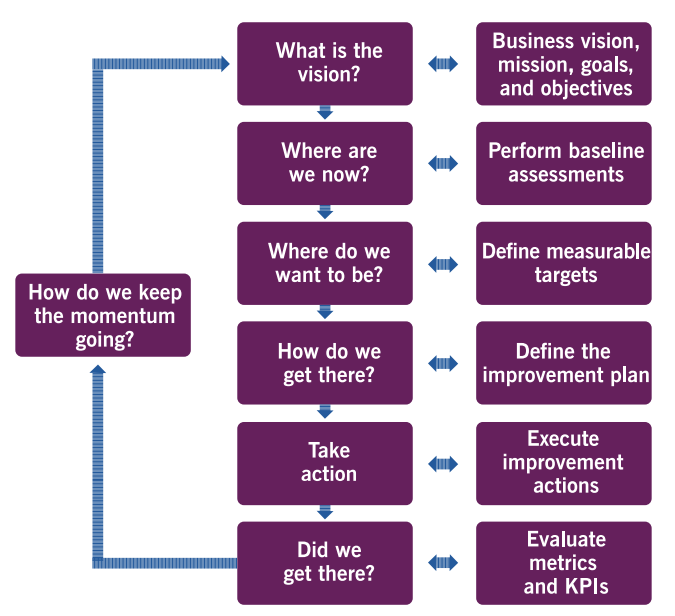
\includegraphics[width=11cm]{img/continual_improvement.png}
        \end{center}
        \caption{Model průběžného vylepšování dle ITIL \parencite[s.~24]{Cartlidge2020}}
        \label{fig:svs_continual_improvement}
    \end{figure} 
    \item Průběžné vylepšení (Continual improvement) - Model kontinuálního vylepšování je v rámci SVS definován jako cyklický řetězec otázek, které jsou úzce propojeny s jednotlivými procesy a metrikami, díky kterým je možné tyto otázky zodpovědět a provést případná vylepšení. Schéma celého řetězce je znázorněno na obrázku \ref{fig:svs_continual_improvement}.
\end{compactitem}

    \begin{table}[h]
        \scriptsize
        \begin{tabularx}{\textwidth}{100X}
            \toprule
                Obecné manažerské postupy & Postupy managementu služeb & Postupy technického managementu \\
             \midrule
                Architecture management & Availability management & Deployment management \\
                Continual improvement & Business analysis & Infrastructure and platform management \\
                Information security management & Capacity and performance & Software development and management \\
                Knowledge management & Change enablement  \\
                Measurement and reporting & Incident management  \\
                Organizational change management & IT asset management  \\
                Portfolio management & Monitoring and event management  \\
                Project management & Problem management  \\
                Relationship management & Release management \\
                Risk management & Service catalogue management \\
                Service financial management & Service configuration management \\
                Strategy management & Service continuity management \\
                Supplier management & Service design \\
                Workforce and talent management & Service desk \\
                Service level management \\
                Service request management \\
                Service validation and testing \\
            \bottomrule
        \end{tabularx}
        \caption{Manažerské postupy dle ITIL \parencite[s.~22]{Cartlidge2020}}
        \label{tab:management_practices_ITIL}
    \end{table}

\chapter{DWH v rámci Masarykovy univerzity}
Masarykova univerzita generuje, jako každá srovnatelně velká instituce, velké množství provozních dat, která jsou však roztříštěna mezi jednotlivými odděleními a to v různých, často vzájemně nekompatibilních formátech. Vzhledem k tomuto stavu, je velmi komplikované tato data jakkoliv využívat , což vedlo k rozhodnutí  vybudovat v rámci univerzity datový sklad, jehož cílem bylo vytvoření jednotného úložiště již zpracovaných dat,  které lze následně využít pro analytické nástroje, které následně pomocí automaticky vytvářených reportů umožňují a zefektivnění  procesů souvisejících s řízením univerzity a poskytnutí dobré startovní pozice k dosáhnutí stavu daty řízené univerzity \footnote{Data Driven University}, zlepšení jejího běžného provozu a v neposlední řadě také poskytnutí lepší podpory podpory výuky.

\section{Služba datového skladu (?)}
Datový sklad je na univerzitě provozován jako služba, která je dle frameworku ITIL v3 definována jako \emph{způsob doručení zákazníkem požadované hodnoty za pomocí výstupů, kterých chce zákazník dosáhnout bez nutnosti vlastnictví specifických nákladů a rizik.} \parencite{SyFvQA11lk1OaIec}

Účel služby datového skladu je dle její webové stránky \footnote{viz. https://it.muni.cz/sluzby/datovy-sklad-na-mu} poskytnutí nástroje, který je schopen sbírat data z různých zdrojů, provést jejich standardizaci a následně je tranformované poskytnout buď ve formě prostých dat, které si může uživatel - zákazník dále dle potřeby zpracovat a nebo ve formě již zpracovaných reportů, které poskytují informace. 

Služba datového skladu má v zásadě dva primární cíle a to:
\paragraph{Automatizace rutinních procesů} kdy je možné velmi zefektivnit pravidelně generovaná data a reporty, jejichž tvorba může být vzhledem k fragmentaci dat časově náročná. 
\paragraph{Podpora rozhodovacích procesů} v rámci které je má poskytnout možnosti sesbírat a zpracovat data, které je následně možné využít pro zefektivnění rozhodovacích procesů. Data pocházející z datového skladu budou s největší pravděpodobností vyšší kvalitu, než data která byla zpracována ručně.

\subsection{Proces zavádění služby datového skladu}

\subsection{Zakládací listina}

\subsection{Procesy}
\paragraph{Uživatel}

\paragraph{Provozovatel}






\section{Technické řešení}
Z výše uvedených konceptů jednotných datových úložišť byl jako nejvhodnější zvolen koncept klasického datového skladu. Ten je v rámci již fungující organizace implementačně jednodušší, neboť se do datového skladu nahrávají jen potřebná data, zatímco například v případě konceptu Data lake, by bylo nutné řešit extrakci dat ze všech podružných systému a pracovišť mnohem komplexněji, neboť cílem většinou bývá centralizace dat ze všech podružných systémů, pracovišť atp. do jednoho místa, což je v případě tak velké organizace jako je Masarykova univerzita velmi problematické. 

Klasický datový sklad není problém postupně rozšiřovat o další data, která jsou požadovaná pro analýzu a případně není problém postupně přecházet na komplexnější architekturu, jako je například Data Lakehouse.

Příslušný datový sklad byl implementován na jaře 2022 za pomocí externí dodavatelské společnosti specializující se na implementaci datových skladů a je postaven zejména na technologií společnosti Microsoft, jeho rámcové schéma je vyobrazeno na obrázku \ref{fig:dwh_muni}

    \begin{figure}[t]
        \begin{center}
            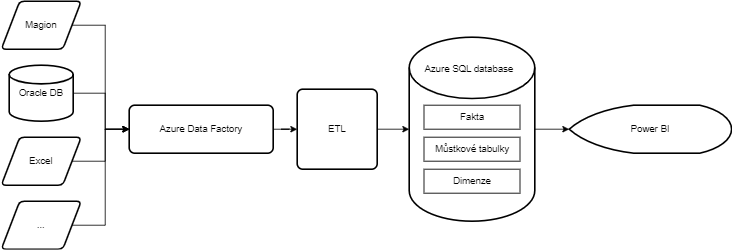
\includegraphics[width=11cm]{img/dwh_muni.png}
        \end{center}
        \caption{Schéma datového skladu MUNI. Vlastní zpracování}
        \label{fig:dwh_muni}
    \end{figure} 
    
Jak je vidět na zmíněném schématu, prvotní sběr dat probíhá pomocí nástroje \emph{Azure data factory}, což je nástroj určený k automatizovanému sběru dat z vícero zdrojů. Za tímto účelem je připojen ke všem potřebným zdrojům, mezi které patří například databázový systém Oracle DB, informační systém Magion a nebo například excelové soubory generované jednotlivými odděleními univerzity. Data z těchto zdrojů jsou pomocí tohoto nástroje pravidelně ve 24 hodinových intervalech extrahována a ukládána na STAGE server, který je realizován v režimu \emph{on premise server}\footnote{Jedná se o server zpravovaný samotnou univerzitou} přímo v prostředí Masarykovy univerzity. Na tomto serveru jsou data uložena v nezpracované formě ve formátu takzvaných snímků \footnote{angl. snapshot}.

Jak je vyobrazeno na schématu, dalším krokem je pak pak proces samotného zpracování dat, což zajišťuje ETL proces, který data patřičně vyčistí a vyfiltruje a to tak, aby byla uložena pouze relevantní data v dostatečné kvalitě. Data jsou následně transformována do podoby, kterou je možné uložit do cloudového úložiště, kterým je v tomto případě Azure SQL databáze\footnote{https://azure.microsoft.com/en-us/pricing/details/azure-sql-database/single/}, což je relační databáze obohacená o inteligentní funkce, které jsou schopny automaticky automaticky upravovat její výkon.

Data jsou v tomto případě uložena ve formě datového schématu zvaného hvězda, který pracuje se třemi druhy tabulek, kterými jsou tabulky obsahující samotná fakta, tedy informace o jednotlivých záznamech, dále tabulky obsahující jednotlivé dimenze, dle kterých je možné data třídit a takzvané můstkové tabulky, které propojují fakta s dimenzemi. 

Data v této podobě je pak již možné přímo zpracovávat analytickými nástroji, jako je například analytický a vizualizační nástroj PowerBI, který je možné připojit přímo na databázi datového skladu, čímž je vždy zajištěna aktuálnost dat. Pomocí nástroje PowerBI lze následně data dále upravovat, vytvářet kontingenční tabulky nebo filtry a následně výsledky vizualizovat pomocí vhodných tabulek, grafů atp. ve formě uživatelských reportů. Tyto reporty lze následně velmi snadno sdílet, neboť je možné je uveřejnit například ve formě webové stránky.

Na tomto datovém skladě je v současnosti již implementováno několik uživatelských aplikací, jako je například interaktivní report využití studoven, který na základě dostupných dat pocházejících z Oracle DB a dále pak z například interních monitorovacích turniketů, vizualizuje ve formě takzvané heatmapy vytíženost jednotlivých studoven  a je z něj tak možné vysledovat, které studovny jsou nejvíce vytížené a v kterou dobu. 

Dalším z příkladu využití datového skladu v rámci Masarykovy univerzity je pak manažerský report pracující s ekonomickými daty centra RECETOX\footnote{z angl .Research Centre for Toxic Compounds in the Environment}. Tento report má jako primární úkol poskytnout podklady pro management, které se týkají lidských zdrojů a jejich úvazků na jednotlivých projektech v rámci centra. Report je  založen na datech pocházejících primárně se informačního systému Magion, které mají formu excelových souborů a před samotným nahráním do datového skladu procházejí manuální úpravou. Automatická tvorba tohoto reportu šetří přibližně 75\% manuální práce, kterou bylo potřeba vynaložit před automatizací.


\section{Zpracovávaný usecase - provozně ekonomická data}
dasdasd

\section{Evaluace a optimalizace procesu}
sadasdasd

\chapter{Aplikační část}
dasdasd

\chapter{Zpracovávaný usecase}
asdasd

\section{Technické řešení}
\subsection{Technické řešení DWH}
asdasd
\subsection{Usecase}
sdas

\section{Návrh implementačního procesu}
\section{Zavedení}

\chapter{Závěr}
\section{Diskuse výsledků práce}
\subsection{Teoretická část}
\subsection{Aplikační část}
\section{Konec}

\printbibliography[heading=bibintoc] %% Print the bibliography.

  \makeatletter\thesis@blocks@clear\makeatother
  \phantomsection %% Print the index and insert it into the
  \addcontentsline{toc}{chapter}{\indexname} %% table of contents.
  \printindex

\appendix %% Start the appendices.
\chapter{An appendix}
Here you can insert the appendices of your thesis.

\end{document}
